\begin{frame}{RTDroid - Prestazioni}
	\only<2>{
		\centering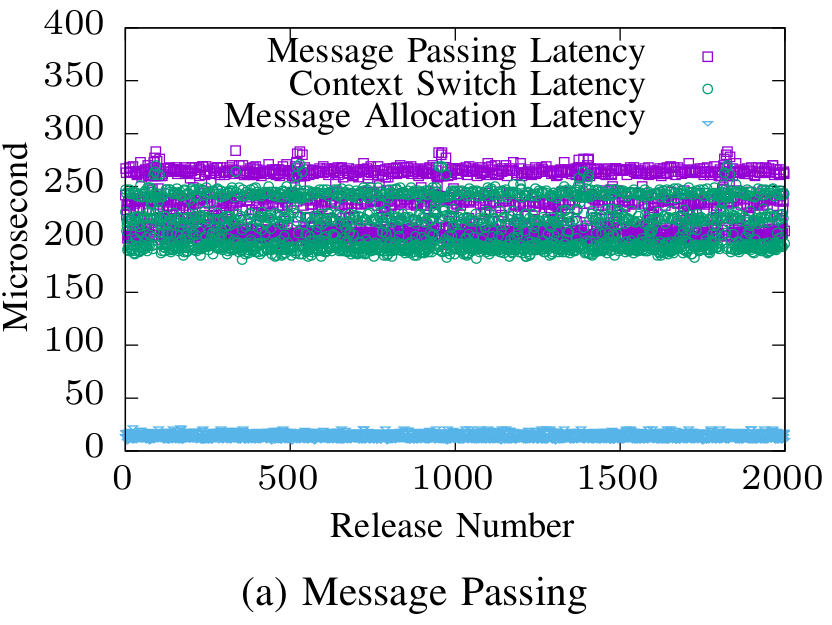
\includegraphics[scale=0.3]{message}
	}

	\only<3>{
		\centering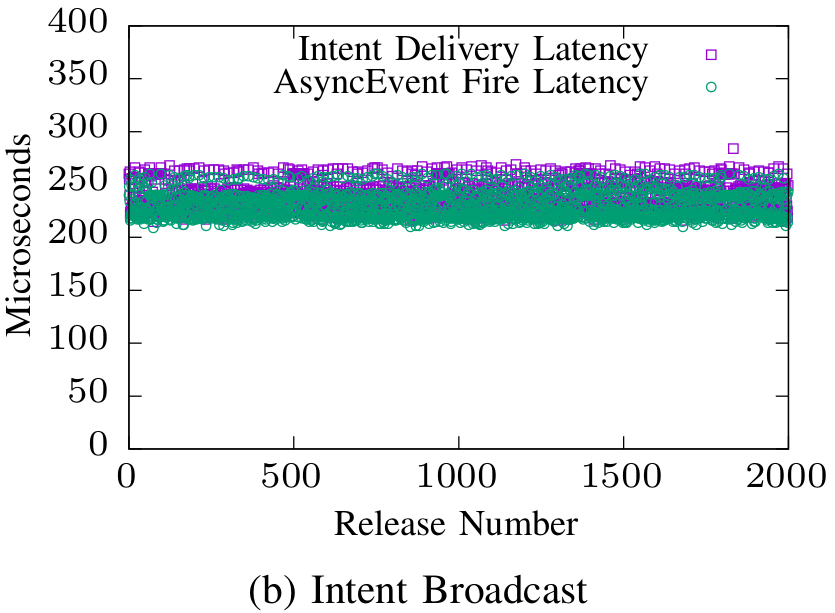
\includegraphics[scale=0.3]{broadcast}
	}
	
	\only<4>{
		\centering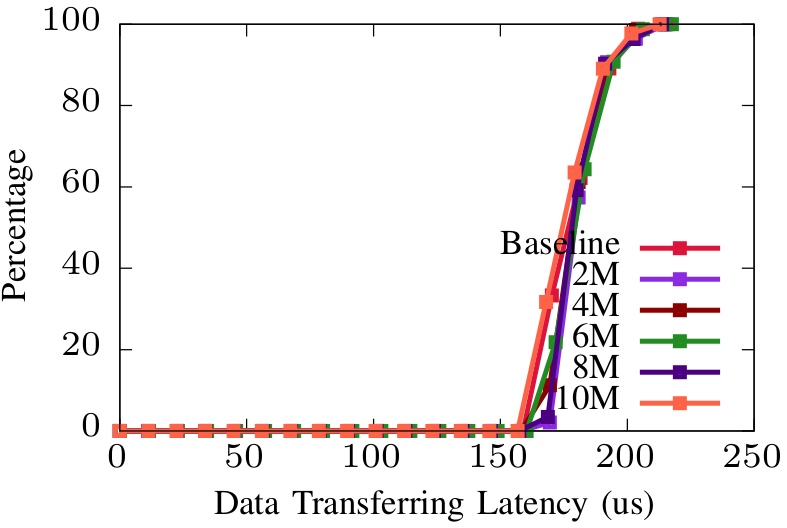
\includegraphics[scale=0.3]{cdfBulk}
	}

	\only<1>{
		\begin{itemize}
			\item Test condotti generando interferenza non real-time
			\begin{itemize}
				\item \textbf{Heap}: allocazione di 512 KB ogni 200 $ms$
				\item \textbf{Calcolo} di $\pi$ ogni 200 $ms$
				\item \textbf{Messaggio} a bassa priorità inviato ogni 200 $ms$
			\end{itemize}
			\item Due thread real-time coinvolti, un sender e un receiver
			\item La latenza rilevata è estremamente limitata
			\begin{itemize}
				\item Le performance sono stabili e prevedibili
			\end{itemize}
		\end{itemize}
	}
\end{frame}